\documentclass[11pt]{report}
% packages
% Fran Burstall's Bath thesis package
\usepackage{baththesis}
\usepackage{amssymb} %for Blackboard bold etc \usepackage{graphicx} %for including eps graphics % front matter
\usepackage[pdftex]{graphicx} % To include pictures
\usepackage{caption}
\usepackage{subcaption} % To use subfigures with subcaptions
\usepackage{url}
\usepackage{amsmath} % Equations
\usepackage{txfonts}
\setlength{\parskip}{0.9em} %Paragraph spacing
\usepackage{pgfgantt}
\usepackage{cite}
\usepackage{csquotes}
\usepackage{multirow}
\usepackage{hhline} % Double lines in tables
\usepackage[ruled]{algorithm2e} % Algorithms 
\renewcommand*{\mkcitation}[1]{ #1}
\usepackage{listings} % For C++ code
\lstset{language=C++,
                basicstyle=\scriptsize,
                keywordstyle=\color{blue}\ttfamily,
                stringstyle=\color{red}\ttfamily,
                commentstyle=\color{green}\ttfamily,
                morecomment=[l][\color{magenta}]{\#},
                showstringspaces=false
}

\newcommand{\phim}{\mathbf{\phi}}
\newcommand{\X}{\mathbf{X}}
\newcommand{\x}{\mathbf{x}}
\newcommand{\Y}{\mathbf{Y}}
\newcommand{\y}{\mathbf{y}}
\newcommand{\w}{\mathbf{w}}
\newcommand{\Z}{\mathbf{Z}}
\newcommand{\z}{\mathbf{z}}
\newcommand{\h}{\mathbf{h}}
\newcommand{\omegam}{\boldsymbol{\omega}}
\newcommand{\deltax}{\left \|  \Delta x \right \|}
\newcommand{\lxo}{\lambda, \x, \omegam}
\newcommand{\C}{\,^{\circ}{\rm C}}
\newcommand{\Maya}{Maya\textsuperscript\textregistered~}
\newcommand{\MentalRay}{Mental Ray\textsuperscript\textregistered~}
\newcommand{\Matlab}{Matlab\textsuperscript\textregistered~}

%\usepackage[hidelinks]{hyperref} % Adds references links without color
\usepackage{hyperref} % Adds references links with color
\usepackage{xcolor}
\hypersetup{
    colorlinks,
    linkcolor={red!50!black},
    citecolor={blue!50!black},
    urlcolor={blue!80!black}
}

\DeclareMathOperator*{\argmin}{arg\,min}
\DeclareMathOperator*{\argmax}{arg\,max}

\title{Realistic fire rendering} \author{Garoe Dorta-Perez}
%\degree{Doctor of Philosophy}
\unit{ CM50170 - Research project }
\department{} 
\degreemonthyear{August 2015}
\norestrictions

% Write here the section you are working on to compile only that one
% You can write more than one section separated by comma
% Comment to compile all
% \includeonly{conclusions} 


\begin{document}

\maketitle

{\hypersetup{linkcolor=black} % Set color back to black
\tableofcontents
}

%------------------------------------------------------------------------------
\chapter{Introduction}
\label{ch:introduction}
\textquote{\textit{A case that can be made for fire being, next to the life process, the most
complex of phenomena to understand}.} - Hoyt Hottle

For centuries humans has been attracted to fire due to its attractive presence and its dangerous nature.
Understanding and simulating combustion phenomena has many applications, such as in the film and computer games industries, where it is widely use in visual effects; or in the engineering community, where the modelling of combustion in engines or fire safety evaluations are frequently demanded.
Computer generated examples include a particle-based technique by~\cite{Reeves:1983} which was used in the Star Trek II film, parametric curves were used to drive the flames in the film Shrek~\cite{Lamorlette:2002} and, the more recent work of~\cite{Horvath:2009} based on 2D screen projection for the film Harry Potter and the Deathly Hallows.
In these and in many other applications, using real flames is an expensive and hazardous endeavour.


Fire can be modelled as a fluid, however its behaviour more complex, due to its multiphase flow, chemical reactions and radiative heat transport, than other fluids, such as water or smoke, which the computer graphics community have intensively researched.
As a result of the aforementioned complexity and the interdisciplinary nature of the problem, fire simulation is still an open problem in computer graphics.

A great deal of work done in the area has sacrificed complexity for interactiveness, therefore producing simplified models which hope to deceit the observer by exploiting the chaotic essence in fire motion.
Nevertheless, physically-based simulations incorporate the intrinsic processes that occur in a combustion scenario:

\begin{description}
\item[Flame motion:]
\item[Fuel erosion:] when the fuel reaches a certain temperature, it is vaporized into a gaseous state, which rises under the influence of buoyancy.
\item[Black body radiation:] the chemical species present in the fuel and the byproducts of the combustions emit energy in various wavelengths.
\end{description}

In order to be able to produce a realistic result, all of the preceding characteristics have to be taken into consideration.

%------------------------------------------------------------------------------
\chapter{Previous Work}
\label{ch:previous_work}

In order to display a realistic fire scene in a computer generated world two differentiated stages are needed.
Firstly, the fire dynamics have to be collected, this can either be done through a data capture session or simulated using a fluid solvers.
Secondly, the previously gathered data is to be visualized on the screen using some rendering technique.

\section{Simulation}
\label{sec:simulation}

Since fire is a multiphase fluid phenomena, it is worthwhile to do a short overview on the main fluid simulation techniques.
Standard fluid simulation has been traditionally geared towards water, nevertheless fire solvers are directly based on such methods.

\section{Fire Simulation}
\label{sec:fire_simulation}

\textbf{Particle-based methods} were the first approach to simulate the visual animation of fire.
A number of particles are emitted from certain locations, each particle has a set of attributes such as shape, velocity, color or lifetime.
The first model with particle systems was presented by~\cite{Reeves:1983}, the particles speed and colour were perturbed with a Gaussian noise at each time step, and the colour was subject to an additional linear perturbation on its lifetime.
Two particle systems were used in a hierarchy, one would control fire spread and the other a single explosion effect.
An extension was proposed by~\cite{Perry:1994}, the authors modified the particle system such that each particle shape would be defined by a series of non-overlapping coplanar triangles.
The transparency of would increase towards the outer vertices, thus providing an improved visual effect.


\textbf{Noise-based methods} focus on synthesizing the high fluctuation present in fire procedurally.
The objective is to approximate the turbulence present in fire with an appropriate statistical model.
Using a variation of Perlin noise, ~\cite{Perlin:1985} presented images of a corona of flames.
However, the method is limited to 2D, where the color is a combination of non-linear arbitrary functions.
This work was extended by~\cite{Perlin:1989} to 3D, where they use volumetric rendering to achieve improved results.

\subsection{Geometry skeleton}

\subsection{Data driven}

\subsection{Physically based}

\subsection{High-speed combustions}

\subsection{Other}
	Erosion and sound paper


%\subsection{Smoke Simulation}
%\label{sec:smoke_simulation}


\section{Rendering}
\label{sec:rendering}


\subsection{Raster-Based}
\label{sec:raster_based}


\subsection{Ray-Tracing-Based}
\label{sec:ray_tracing_based}


\cite{Pegoraro:2006} says ...

%------------------------------------------------------------------------------
\chapter{Methodology}
\label{ch:methodology}

Not only explain in more detail every equation, what it means, comparison with other papers and ideally improvements or were it fails at least.
Should I explain what is and how to do ray marching? What is the spectrum? How to integrate it to RGB coefficients?

\section{Radiative Transport Equation}
\label{sec:radiative_transport_equation}

The Radiative Transport Equation (RTE) models the variation of spectral radiance in the medium $L(\lxo)$, where $\lambda$ is a given wavelength in $m$, $\x$ is the point of interest in space, and $\omegam$ is a vector that points towards the viewing direction.
The RTE is defined as

\begin{equation}
\begin{split}
(\omega \nabla) L(\lxo) = &- \sigma_a(\lambda, \x) L(\lxo) + \sigma_a(\lambda, \x) L_e(\lxo) \\
&- \sigma_s(\lambda, \x) L(\lxo) + \sigma_s(\lambda, \x) L_i(\lxo),
\end{split}
\end{equation}

where $L_i$ is defined as

\begin{equation}
L_i(\lxo) = \int_{4 \pi} L(\lxo_i) \Phi (\lambda, \omegam, \omegam_i) d \omegam_i,
\end{equation}

where $\sigma_a$ is an absorption coefficient, $\sigma_s$ is a scattering coefficient, $L_e$ is the emitted spectral radiance at the point, $L_i$ is the in-scattering radiance and $\Phi$ is a scattering function.
In order to get an analytical solution to the aforementioned equation, the properties of the medium are assumed to be homogeneous over a small segment $\deltax$ in space,

\begin{equation}
\begin{split}
L(\lambda, \x + \Delta\x, \omegam) &= e^{-\sigma_t(\lambda, \x) \deltax} L(\lxo) +  \\
& (1 - e^{-\sigma_t(\lambda, \x) \deltax} ) \frac{\sigma_a(\lambda, \x) L_e(\lxo) + \sigma_s(\lambda, \x) L_i(\lxo)}{\sigma_t(\lambda, \x)},
\end{split}
\end{equation}

where $\sigma_t = \sigma_a + \sigma_s$ is the extinction coefficient.

\section{Scattering}
\label{sec:scattering}


\section{Soot Absorption}
\label{sec:soot_absorption}


\section{Black Body Radiation}
\label{sec:black_body_radiation}


\section{Emission From Chemical Species}
\label{sec:emission_from_chemical_species}



\section{Refraction}
\label{sec:refraction}



\section{Visual Adaptation}
\label{sec:visual_adaptation}




%------------------------------------------------------------------------------
\chapter{Implementation details}
\label{ch:implementation_details}

In this chapter we will explain how to use the shaders which have been implemented and the differences between the theoretical pipeline explained in Chapter~\ref{ch:methodology} and the actual software implementation.
An overview of the pipeline is shown in Figure~\ref{fig:pipeline_simplified}, note that the modules in grey are not present in the software.

\begin{figure}[htbp!]
	\centering
	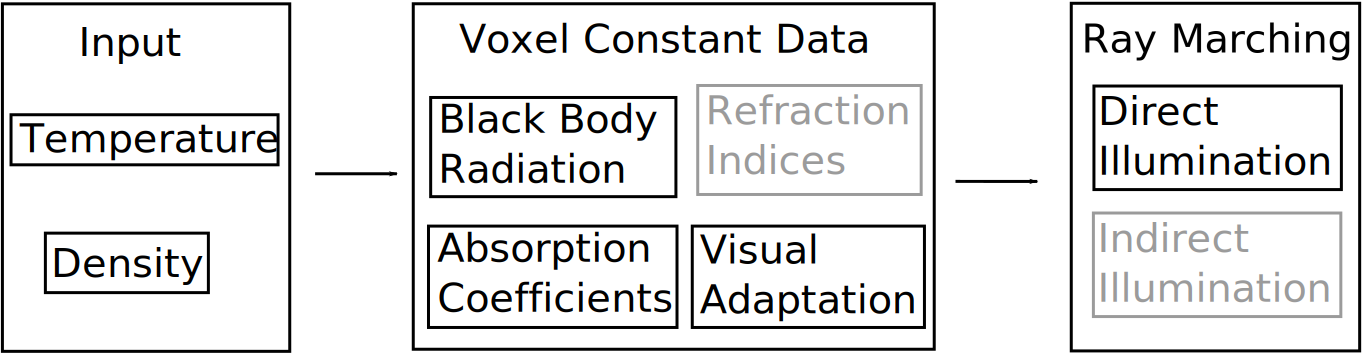
\includegraphics[width=\textwidth]{img/pipeline_simplified}
	\caption{An overview of the implemented fire rendering pipeline.}
	\label{fig:pipeline_simplified}
\end{figure}

The implementation of the model was realised with several shaders for \MentalRay to be used in \Mayash.
Using a rendering engine like \MentalRaysh, which provides the basic functionality needed for ray tracing, means that the code is implemented using a predefined abstraction layer, thus reducing bugs in the code and increasing the programmer's productivity.
The integration with \Maya is desirable, as the software gives the user an intuitive environment in which to create complex scenes, that are compatible with off-the-shelf effects like cloth or fluid simulations. 

\section{Application Overview}
\label{sec:application_overview}

\begin{figure}[htpb!]
        \centering
        \begin{subfigure}[t]{\textwidth}
                \includegraphics[width=\textwidth]{img/application_example}
                \caption{Test scene, note on the right the shader interface.}
                \label{fig:application_example}
        \end{subfigure}%
        \\  %add desired spacing between images, e. g. ~, \quad, \qquad, \hfill etc.
          %(or a blank line to force the subfigure onto a new line)
        \begin{subfigure}[t]{\textwidth}
                \includegraphics[width=\textwidth]{img/application_example_render}
                \caption{Low quality rendered image from the scene above.}
                \label{fig:application_example_render}
        \end{subfigure}
        \caption{Application interface in \Mayash.}
        \label{fig:application_example_full}
\end{figure}

Figure~\ref{fig:application_example} shows the \Maya interface for our shaders in a test scene.
From the user view point the volumetric data is enclosed in a cube, that can be manipulated like any other object in the scene.
The GUI for the shader includes two input files and  sliders for the numeric parameters. 
The scene rendered from the camera viewpoint is shown in Figure~\ref{fig:application_example_render}.

The model chosen for our inputs is that of a three-dimensional voxel dataset, a cube in space is uniformly divided and a value is stored for each voxel.
This data in the voxel is either a soot density estimate for the \textit{fire volume shader} or a temperature estimate for the \textit{fire light shader}.
Three file formats for floating point data are supported, dense or sparse values in plain ASCII files, and sparse RGBA values in binary files, as shown in Figure~\ref{fig:file_format}.
In the ASCII dense format, the first line of the file are three integers, separated by spaces, declaring the width, height and depth of the data, followed by $w \times h \times d$ lines with floating point values.
The ASCII sparse format, has two extra parameters in the first line, $c$ is the number of data points in the file and $b$ is the default value for any voxel that is not specified in the file.
Each data line has the $x,y,z$ coordinates and the data value separated by spaces.
The RGBA binary sparse format starts with a 4 bytes integer declaring how many data points are in the file, each voxel has its coordinates $x,y,z$ as 4 bytes integers and a RGBA colour, where each channel is encoded with an 8 bytes floating point value.
Any voxel that is not included in the file is considered to be initialized to zero. 

\begin{figure}[htpb!]
        \centering
        \begin{subfigure}[t]{0.16\textwidth}
                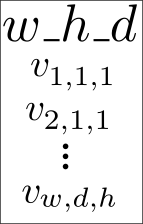
\includegraphics[width=\textwidth]{img/file_format_ascii_dense}
                \caption{ASCII dense (*.vol).}
                \label{fig:file_format_ascii_dense}
        \end{subfigure}%
        ~ %add desired spacing between images, e. g. ~, \quad, \qquad, \hfill etc.
          %(or a blank line to force the subfigure onto a new line)
        \begin{subfigure}[t]{0.24\textwidth}
                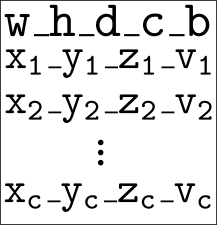
\includegraphics[width=\textwidth]{img/file_format_ascii_sparse}
                \caption{ASCII sparse (*.uintah).}
                \label{fig:file_format_ascii_sparse}
        \end{subfigure}
        ~ %add desired spacing between images, e. g. ~, \quad, \qquad, \hfill etc.
          %(or a blank line to force the subfigure onto a new line)
        \begin{subfigure}[t]{0.2256\textwidth}
                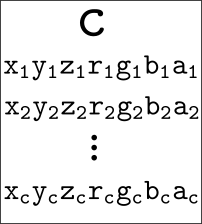
\includegraphics[width=\textwidth]{img/file_format_binary}
                \caption{Binary sparse (*.raw).}
                \label{fig:file_format_binary}
        \end{subfigure}
        \caption{Suported file formats, $\_$ represent the character space.}
        \label{fig:file_format}
\end{figure}

\section{\MentalRay Rendering Approach}
\label{sec:mental_ray_rendering_approach}

\MentalRay approach to solving the rendering equation is based on path tracing, as shown in Figure~\ref{fig:mental_ray_model}, for each pixel in the camera view, an eye ray will be shot in the scene.
On an intersection with an object in the scene, its material shader will be called, this shader will shoot a light ray for each light in the scene, which in effect calls the light shader of the given light.
In order to compute the irradiance at the intersection point, the light shader will trace a shadow ray from the light to the intersection point.
Eventually, the material shader will compute the final colour with the information received from the light shader. 

\begin{figure}[htbp!]
\centering
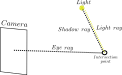
\includegraphics[width=0.8\textwidth]{img/mental_ray_model}
	\caption{\MentalRay simple ray casting example.}
	\label{fig:mental_ray_model}
\end{figure}

Under this assumptions, the steps required to solve the RTE, Equation~\ref{eq:rte_solution_paper}, are:

\begin{enumerate}
\item Shoot a ray from the eye into the scene.
\item If the ray intersects the fire volume, perform ray marching in the volume.
	\begin{enumerate}
	\item Compute direct illumination at the current point.
		\begin{enumerate}
		\item Sample all the lights $\rightarrow L_e$
		\item Attenuate each with its own absorption coefficient $\rightarrow \left( 1 - e^{-\sigma_a} \right) L_e$
		\end{enumerate}	
	{\color{gray} \item Compute indirect illumination at the current point $\rightarrow \sigma_s L_i$
		\begin{enumerate}
		\item Use phase function to get the scattered light distribution $\rightarrow \Phi$
		\end{enumerate}}
	\item Add current contribution to accumulated color $\rightarrow e^{-\sigma_t}L + \left( 1 - e^{-\sigma_a} \right) L_e$
	\item Advance to next point in ray marching $\rightarrow \x = \x + \Delta \x$
		\begin{enumerate}
		{\color{gray} \item Change ray direction using refraction index $\rightarrow \Delta \x = refract (\Delta \x)$}
		\end{enumerate}	
	\end{enumerate}
\end{enumerate}

\section{Simplifications}
\label{sec:simplifications}

Equation~\ref{eq:rte_solution_paper} provides a radiance value $L(\lambda, \x + \Delta\x, \omegam)$ for the next march increment, however it is more intuitive to think about the final radiance $L(\lambda, \x, \omegam)$ for the first intersection point.
The radiance at the interest point is given by 

\begin{equation}
\begin{split}
L(\lambda, \x, \omegam) &= e^{-\sigma_t(\lambda, \x) \deltax} L(\lambda, \x + \Delta\x, \omegam) +  \\
& \left(1 - e^{-\sigma_t(\lambda, \x) \deltax} \right) \frac{\sigma_a(\lambda, \x) L_e(\lxo) + \sigma_s(\lambda, \x) L_i(\lxo)}{\sigma_t(\lambda, \x)}.
\end{split}
\end{equation}

In fire phenomena the effect of scattered light in the final image is practically imperceptible~\cite{Pegoraro:2006}.
Intuitively, it means that as the medium is highly emissive and thin, most of the emitted photons have their initial paths unaltered.
The scattering directions $\omegam_i$ are in essence sampling directions over a sphere of scattered light $L_i$.
In practice, the simplification will significantly decrease rendering time, as $\omegam_i$ would have to be sampled by means of a computationally expensive Monte Carlo approximation. 
Exploiting that prior knowledge, the scattering contributions can be safely ignored by setting $\sigma_s = 0$, which simplifies the previous equation to

\begin{equation}
L(\lambda, \x, \omegam) = e^{-\sigma_a(\lambda, \x) \deltax} L(\lambda, x + \Delta\x, \omegam) +  \left(1 - e^{-\sigma_a(\lambda, \x) \deltax} \right) L_e(\lxo).
\label{eq:rte_simplified}
\end{equation}

A visual representation of the implications of the aforementioned simplification is shown in Figure~\ref{fig:ray_marching}.
Note that a single point light is used in the diagram to avoid clutter, yet in our implementation there is a point light located at the centre of each voxel whose temperature is high enough to be emissive.
The non-linear trajectories of the photons, of the rays in practice, due to varying refraction indices in the media were also outside of the scope of this project.
Deformations produced by the refraction phenomena can be noticeable, however there are important simplifications in the implementation if we choose to ignore them.
Namely, we can reduce the recursiveness significantly, instead of starting in the first intersection and recursively solving the equation, we can start from the end point and accumulate the result backwards with a loop, as computing the end point in this situation is trivial.

\begin{figure}[htbp!]
	\centering
	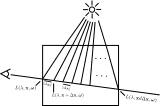
\includegraphics[width=0.8\textwidth]{img/ray_marching}
	\caption{Calculating the illumination values for samples along a ray.}
	\label{fig:ray_marching}
\end{figure}

\section{Shaders Overview}
\label{sec:shaders_overview}

Given the complexity of the task at hand, a modular architecture for the system was chosen.
As depicted in Figure~\ref{fig:shaders_diagram}, the main shader (Fire Volume) delegates the computation of several values to other auxiliary shaders.   
The temperature and density shaders read the raw input values, the emission and absorption shaders compute respectively, black body radiation and absorption coefficients.
The fire light shader manages light rays by precomputing and sampling the emitted light $L_e$.
The fire volume shader is in charge of including the absorption coefficient with shadow rays, and to perform the main ray marching computations, eye rays. 

\begin{figure}[htbp!]
	\centering
	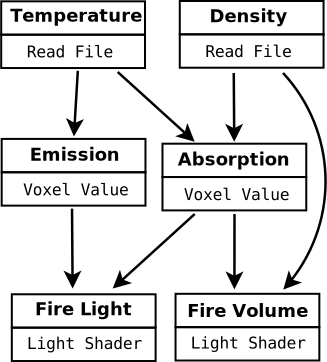
\includegraphics[width=0.4\textwidth]{img/shaders_diagram}
	\caption{Diagram depicting the shaders and their interconnections.}
	\label{fig:shaders_diagram}
\end{figure}

\begin{figure}[htpb!]
        \centering
        \begin{subfigure}[b]{0.7\textwidth}
                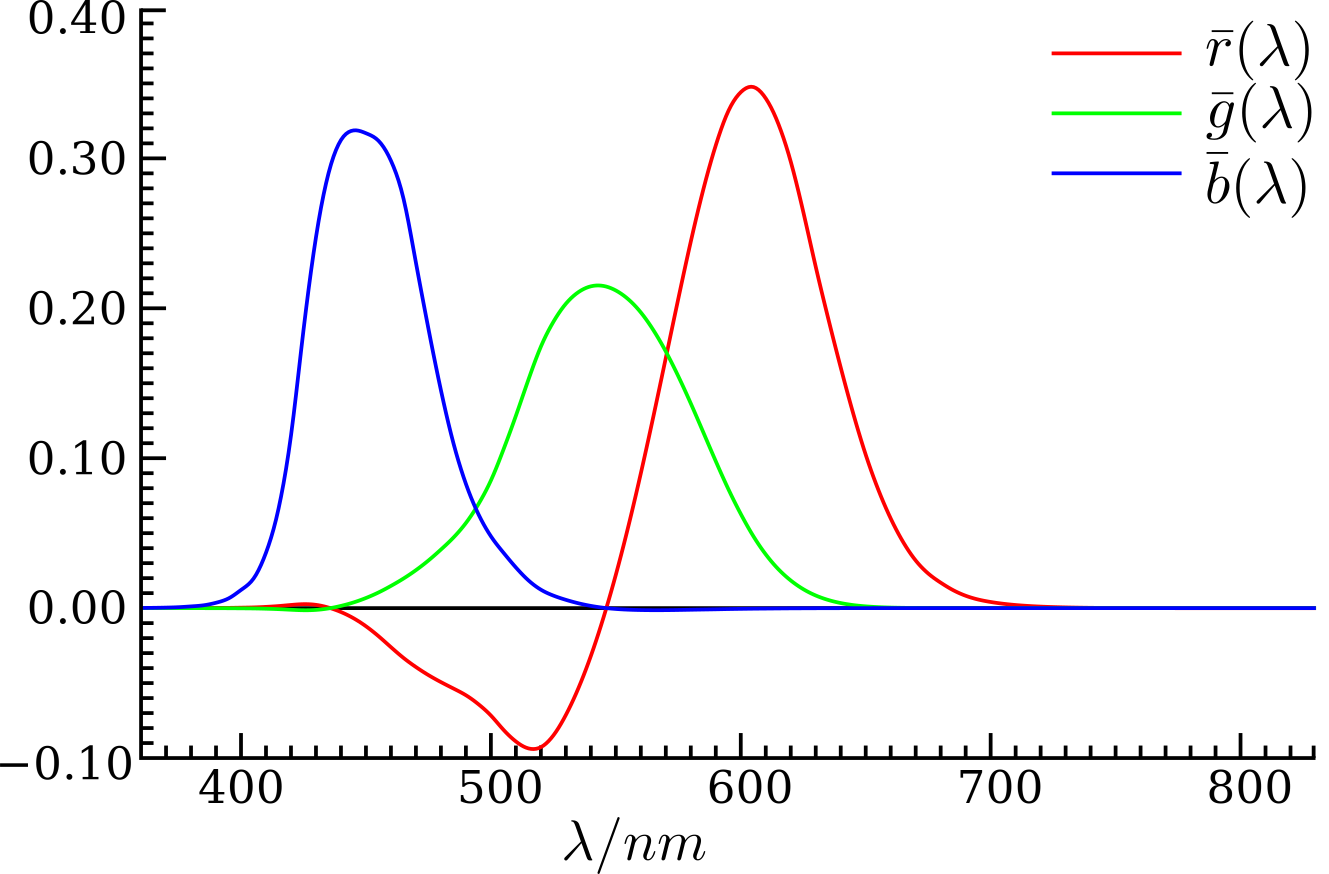
\includegraphics[width=\textwidth]{img/CIE_RGB}
                \caption{Spectral tristimulus values for CIE RGB~\cite{CIE_RGB}.}
                \label{fig:cie_rgb}
        \end{subfigure}%
        \quad %add desired spacing between images, e. g. ~, \quad, \qquad, \hfill etc.
          %(or a blank line to force the subfigure onto a new line)
        \begin{subfigure}[b]{0.7\textwidth}
                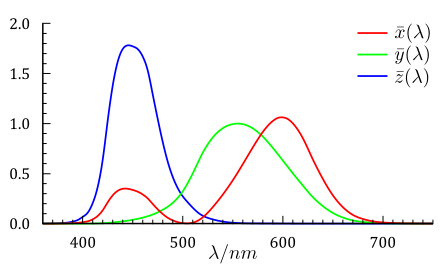
\includegraphics[width=\textwidth]{img/CIE_XYZ}
                \caption{Spectral tristimulus values for CIE XYZ~\cite{CIE_XYZ}.}
                \label{fig:cie_xyz}
        \end{subfigure}
        \caption{Colour matching curves for RGB and XYZ spaces.}
\end{figure}

\section{Spectrum to RGB}
\label{sec:spectrum_to_rgb}

To speed up the render time, all spectrum related computations are integrated at source to RGB coefficients.
Our spectrum class has a number of samples that can be set at compile time, 30 samples were used in all of our renderings.
To compute the absorption coefficients that were introduced in Section~\ref{sec:absorption_coefficients}, data from Table~\ref{tb:soot_absorption_coefficients} is used.
As there is not enough data to compute the 30 spectrum coefficients, a linear interpolation is used to fill the missing values.
RGB coefficients are the standard colour representation in computer screens, however not every colour visible by the human eye can be reproduced in RGB space.
There are further disadvantages inherent to this representation, for example certain colours visible by the human eye would require negative values for the $\bar{r}(\lambda)$ coefficient, as shown in Figure~\ref{fig:cie_rgb}.
The XYZ colour space is built using three sets of imaginary primaries, which have a series of favourable properties.
Any colour which can be seen by the human eye can be represented with some $x(\lambda)$, $y(\lambda)$, $z(\lambda)$ coefficients, the Y channel is equal to the photopic luminous efficiency function $V(\lambda)$, which models the variation of perceived brightness, and as shown in Figure~\ref{fig:cie_xyz}, the coefficients are always positive.

Given a Spectral Power Distribution (SPD) $S(\lambda)$, the $x$, $y$, $z$ coefficients for $S(\lambda)$ in the XYZ space are defined with respect to spectral matching curves $X(\lambda)$, $Y(\lambda)$ and $Z(\lambda)$, such that

\begin{equation}
\begin{split}
x &= \frac{1}{\int Y(\lambda) d\lambda} \int_\lambda S(\lambda) X(\lambda) d\lambda, \\
y &= \frac{1}{\int Y(\lambda) d\lambda} \int_\lambda S(\lambda) Y(\lambda) d\lambda, \\
z &= \frac{1}{\int Y(\lambda) d\lambda} \int_\lambda S(\lambda) Z(\lambda) d\lambda.
\end{split}
\end{equation}

The term $1 / \int Y(\lambda) d\lambda$ is added in each equation to act as a normalization factor for the colour brightness. 
As we are concerned with sampled values on a discrete domain, the integration for XYZ coefficients is approximated by a Riemann sum

\begin{equation}
\begin{split}
x &\approx \frac{1}{\int Y(\lambda) d\lambda} \sum_i X_i c_i, \\
y &\approx \frac{1}{\int Y(\lambda) d\lambda} \sum_i Y_i c_i, \\
z &\approx \frac{1}{\int Y(\lambda) d\lambda} \sum_i Z_i c_i,
\end{split}
\end{equation}

where $c_i$ is the $i^{th}$ coefficient in the SPD, $X_i$ is the area for the corresponding sample range in the $X(\lambda)$ curve and equivalently for $Y_i$ and $Z_i$.
Note that $1 / \left(\int Y(\lambda) d\lambda \right)$, $X_i$, $Y_i$ and $Z_i$ are constants and they can be precomputed for efficiency.
For the Riemann sum, the area under the samples is approximated using piecewise linear interpolation.
The conversion from XYZ to RGB space is performed using

\begin{equation}
\begin{bmatrix}
r \\
g \\
b
\end{bmatrix}
 = 
\begin{bmatrix}
\int R(\lambda) X(\lambda) d\lambda & \int R(\lambda) Y(\lambda) d\lambda & \int R(\lambda) Z(\lambda) d\lambda \\
\int G(\lambda) X(\lambda) d\lambda & \int G(\lambda) Y(\lambda) d\lambda & \int G(\lambda) Z(\lambda) d\lambda \\
\int B(\lambda) X(\lambda) d\lambda & \int B(\lambda) Y(\lambda) d\lambda & \int B(\lambda) Z(\lambda) d\lambda
\end{bmatrix}
\begin{bmatrix}
x \\
y \\
z
\end{bmatrix},
\end{equation}

where $R(\lambda)$, $G(\lambda)$, $B(\lambda)$ are the spectral curves for the red, green and blue colours respectively.
Note that all the factors in the transformation matrix are constants and they can be precomputed for efficiency.

\subsection{Performance considerations}
\label{sec:performance_considerations}

Volumetric data tends to be quite sparse, and usually we are working with volumes of $256 \times 256 \times 256$ voxels, which assuming a 32 bits floating point value per voxel in the density and temperature shader, and three floating point values for the emission and absorption shaders, accumulates respectively to 64 and 192 megabytes of data.
With the shader architecture shown in Figure~\ref{fig:shaders_diagram}, there will be at least two copies of each structure per fire in the scene.
Since a total of 512 megabytes per voxel dataset is unacceptable, we use an open source sparse voxel dataset library~\cite{OpenVDB}.
The sparse data structure reduced the total memory consumption to approximately 20 megabytes per dataset, while increasing the total rendering time by less than 10 seconds on average.

In order to achieve smoother rendering results, a trilinear interpolation is computed in each step in the ray-marching algorithm.
Computing the interpolation smoothed the shape of the flames and reduced the effects of outliers is the input data.
Tricubic interpolation was also considered, however it was discarded due to the significant increase in computational overhead.

Our system follows the recommendations of the \MentalRay API, which allows performance to scale automatically as the number of hardware processors increases.
Batch rendering for animations is also supported, the shaders will automatically choose the correct input files for each frame. 

\section{Visual Adaptation}
\label{sec:visual_adaptation_imp}

The implementation of the eye visual adaptation to the colours in fire, described in Equation~\ref{eq:visual_adaptation} is performed as described in~\cite{Nguyen:2002}, which uses the Von Kries model~\cite{Fairchild:2005} 

\begin{equation}
\begin{split}
\x_a &= \mathbf{M}^{-1} \mathbf{T}_w \mathbf{M} \x_i, \\
\mathbf{l}_{max} &= \mathbf{M} \mathbf{x}_{max}, \\
\mathbf{T}_w &= 
\begin{bmatrix}
1 / l_{max} & 0 & 0\\
0 & 1 / m_{max} & 0\\
0 & 0 & 1 / s_{max}\\
\end{bmatrix}, \\
\mathbf{M} &= 
\begin{bmatrix}
0.4002 & 0.7076 & -0.0808\\
-0.2263 & 1.1653 & 0.0457\\
0 & 0 & 0.9182\\
\end{bmatrix},
\end{split}
\end{equation}

where $\x_a = \left[ x_a, y_a, z_a \right]^{T}$ is a column vector with the XYZ adapted coefficients, $\mathbf{T}_w$ is the Von Kries transformation, $x_{max}$ are the coefficients for the maximum temperature present in the fire,  $\mathbf{l}_{max} = \left[ l_{max}, m_{max}, s_{max} \right]^{T}$ are the LMS coefficients of $x_{max}$, $\mathbf{M}$ is a XYZ to LMS transformation matrix and, $\x_i = \left[ x_i, y_i, z_i \right]^{T}$ is a column vector with the XYZ input coefficients.
The $\mathbf{M}$ matrix is a Hunt-Pointer-Estevez transformation, proposed by~\cite{Hunt:1985}, which has been normalized to the CIE Standard Illuminant D65.
The coefficients for $\mathbf{M}^{-1}$ are not provided in the CIE specification.
Given that $\mathbf{M}$ is a small $3 \times 3$ matrix, the coefficients of $\mathbf{M}^{-1}$ can be evaluated with any of the standard matrix inversion methods, in our case the default algorithm in \Matlab \textit{inv()} function was used, and the output was hard-coded in the shader.
The aforementioned equation is solved in the XYZ space, in order to delay clamping coefficients to RGB as much as possible.

\section{Miscellaneous}
\label{sec:miscellaneous}

\subsection{Utilities}
\label{sec:utilities}

Several auxiliary scripts have been developed in order to aid and provide some automation while using the software.
A bash render script ``render.sh" is provided, this script batch renders a given \Maya scene and creates a video with the output images.

New fuel types can be added to extend the default selection using spectral lines from the NIST database~\cite{Nist}.
A \Matlab script ``save\_nist\_data.m" can be used to download and save new ``.specline" files for new atoms.
Once a new file has been added to the data folder, the files ``fire\_shader.mi" and ``FuelTypes.h" have to be updated to include the name of the new data.

Uintah~\cite{Uintah} is the combustion simulator used by~\cite{Pegoraro:2006} as input for their rendering method.
Detailed instructions for its installation on Ubuntu, how to run examples, as well as scripts to convert from their output data format to a format compatible with the shaders is provided with the source code.

\subsection{Known bugs and workarounds}
\label{sec:known_bugs_and_workarounds}

Batch rendering through the \Maya GUI does not automatically update the input files for the shaders.
A workaround is to use the command line render utility as shown below

\begin{lstlisting}[language=bash,caption={Batch render command}]
$ Render -r mr -perframe -s <start_frame_number> -e <end_frame_number> <path_to_scene_file>
\end{lstlisting}

Saving images, either from batch render or single frame GUI render, will produce unexpected results, normally a completely white output, if the image format natively supports transparency, such as tif, tga or exr.
In order to get consistent results, the scene should be surrounded by solid objects.

Any \Maya scene which uses the shaders should be saved in \Maya ASCII format, ``{\textless}scene{\textgreater}.ma".
The saved files are not platform independent, as the input file names for the shaders use absolute paths.
If the scene is to be opened in a new environment, the file paths have to be modified to match the current locations.

%------------------------------------------------------------------------------
\chapter{Results}
\label{ch:results}

Images everywhere and proper analysis of what the user is seeing, what is failing and why.
Include default Maya fire effect, pictures of fire from the papers mentioned in the previous work section and a historical overview on the improvements in the shaders.

%------------------------------------------------------------------------------
\chapter{Conclusions and Future work}
\label{ch:conclusions}

\section{Conclusions}

\section{Future Work}

An interesting area of future work involves automatically setting the shader parameters for a given scene.
There are at least two paths that be used to give a good parameter estimation, if we have captured data.
The methods are, gradient descent using image derivatives or reconstructing the spectrum which produced the cameras RGB responses.
Both techniques will be explained in greater detail in the Sections~\ref{sec:image_differences} and~\ref{sec:spectrum_reconstruction}.

A common line of work in the computer graphics community is the development of importance sampling for a bxdf rendering models~\cite{Lawrence:2004},~\cite{Ou:2012} and~\cite{Wang:2014}.
The core idea is to sample more often the values that contribute more to the final image, by means of a biased distribution instead of an uniform sampling scheme.
In our implementation the emitted radiance $L_e$ is uniformly sampled, and in the general case the $\omegam_i$ directions for in-scattering light $L_i$ would have been naively sampled as well.
In order to design a ``good" biased distribution, prior knowledge of the location of the important regions is needed. 
For $L_e$ and $L_i$ we have some intuitive insight on were would such regions lie, samples whose origin is close to the interest point should have greater contributions, as the influence of further ones will be diminished by the light distance falloff effect.
Another factor which must be considered is the relative intensity emitted at source by a sample, as it is expected that brighter points will have larger contributions. 

\subsection{Image differences}
\label{sec:image_differences}

Given a ground truth captured image $I_f$, we would like to transform an image $I_0$, rendered with our method, so that it resembles $I_f$.
Formally the transformation is defined as

\begin{equation}
I_{i+1} = t(I_i,~d(I_i,~I_f)),
\end{equation}

where $I_i$ is the image in the $i^{th}$ step, $d$ is an image difference function, and $t$ is a function that transform $I_i$ in the direction of the gradient given by $d$.
There are several terms in the aforementioned equation that can be explored in more detail.
A number of image difference filters have been proposed, such as the Sobel and the Scharr filters.
The transformation function $t$ must convert from image derivatives space, to the physical parameter space that our shaders use, temperature, density, light falloff rate, etc.
The simplest technique to compute the next step in the parameter space would be gradient descent.
As there are several parameters to explore, and their behaviour is non-linear, it is reasonable to expect that the function will have a number of local minima. 
Thus, requiring more advanced optimization methods, such as genetic programming.

\subsection{Spectrum reconstruction}
\label{sec:spectrum_reconstruction}

In a captured image $I_f$, each pixel stores the RGB values that were measured by the sensor at that position.
When the camera is exposed to a spectral signal, the spectrum is collapsed to RGB space using the sensor spectral sensitivity curves for each color, the curves are shown in Figure~\ref{fig:camera_sensitivity}.
In continuous form, the collapsing of the signal is driven by

\begin{figure}[htbp!]
\centering
\includegraphics[width=0.8\textwidth]{img/camera_sensitivity}
	\caption{Spectral sensitivity curves for the sensors in our cameras.}
	\label{fig:camera_sensitivity}
\end{figure}

\begin{equation}
\begin{split}
r &= \int i(\lambda) s_r(\lambda) d \lambda, \\
g &= \int i(\lambda) s_g(\lambda) d \lambda, \\
b &= \int i(\lambda) s_b(\lambda) d \lambda,
\end{split}
\label{eq:spectrum_collapse_cont}
\end{equation}

where $r$, $g$ and $b$ are the output coefficients, $i(\lambda)$ is the input spectrum, $s_r(\lambda)$, $s_g(\lambda)$ and $s_b(\lambda)$ are the spectral sensitivity curves and $\lambda$ is a wavelength number.
Discretized for $n$ samples the previous equation can be written as  

\begin{equation}
\begin{bmatrix}
r \\
g \\
b
\end{bmatrix}
= 
\begin{bmatrix}
s_r(\lambda_0) & s_r(\lambda_1) & \cdots & s_r(\lambda_n) \\
s_g(\lambda_0) & s_g(\lambda_1) & \cdots & s_g(\lambda_n) \\
s_b(\lambda_0) & s_b(\lambda_1) & \cdots & s_b(\lambda_n) 
\end{bmatrix}
\begin{bmatrix}
i(\lambda_0) \\
i(\lambda_1) \\
\vdots \\
i(\lambda_n) 
\end{bmatrix}.
\label{eq:spectrum_collapse_disc}
\end{equation}

If the original signal $i(\lambda)$ were to be reconstructed, the physical parameters could be computed using the equations presented in Chapter~\ref{ch:methodology}.
An image rendered with those parameters would closely resemble the original data.
The main challenge in this situation lies in the highly underconstrained nature of the problem, $n$ unknowns in $i(\lambda)$ are to be solved with only three equations from $r$, $g$ and $b$.
Fortunately, several methods have been proposed,~\cite{Smits:1999},~\cite{Sun2001} and~\cite{Drew:2003}, to compute an approximation of $i(\lambda)$ using optimization techniques with a set of prior constrains, such as smooth spectral curves and spatial coherency within the image.



\newpage
\bibliographystyle{eg-alpha}
\bibliography{fire_rendering}

\end{document}

